\section{The Circular Restricted Three-Body Problem}\label{sec:CR3BP}
When a spacecraft is significantly impacted by the gravitational force of two celestial bodies, the
circular restricted 3-body problem better approximates the spacecraft behavior compared to two-body
problems. Consequently, this investigation employs the CR3BP to model the Earth-Moon and Sun-planet
systems when appropriate. The CR3BP is a time-autonomous model (its dynamics are time-invariant)
that provides insight into some of the dynamical structures present in the system without the
additional complexities of a higher-fidelity ephemeris force model.

\subsection{Equations of Motion}
The CR3BP consists of three primary bodies, two celestial bodies and a massless spacecraft. The two
celestial bodies exert gravitational forces on each other and the satellite; however, the satellite
does not affect the behavior of the other two bodies. All three bodies are treated as point masses
and assumed to move in circular orbits, with a constant angular velocity, around their barycenter
$B$. Assuming that other forces are not acting on the system, $B$ is considered an inertially-fixed
point, and similar to the 2BP, Newton's Laws are expressed relative to that point. Unlike the 2BP
however, there currently is not an analytical solution to represent the dynamics of the CR3BP.
Consequently, all trajectories in the CR3BP must be numerically propagated in time with nonlinear,
coupled equations of motion. It is helpful and common practice to represent and visualize the
equations of motion in a barycentric rotating coordinate frame, $\{\xhat,\yhat,\zhat\}$, indicated
by the dashed lines in \cref{fig:baryFrames} and described in \cref{sec:CoordinateFrames}. In the
rotating frame, the two celestial primaries remain fixed, while the spacecraft moves relative to
them in three-dimensional configuration space. This framework provides a foundational model for
studying complex spacecraft trajectories, leveraging numerical methods to capture the intricate
dynamics of the CR3BP.

A CR3BP system is defined by a single mass ratio $\mu$ that characterizes the gravitational
interactions and forms the basis for deriving the system equations of motion in the barycentric
rotating frame. This parameter is the ratio between the masses of the larger ($m_{1}$) and smaller
($m_{2}$) celestial primaries:
\begin{equation}
    \mu=\frac{m_{2}}{m_{1}+m_{2}}.
    \label{eq:mu}
\end{equation}
In the barycentric rotating frame, $P_{1}$ is located at $x=-\mu$ and $P_{2}$ is
located at $x=1-\mu$. A pseudo-potential function $U$ describes the gravitational forces on the
system expressed in the barycentric rotating frame:
\begin{equation}
    U=\frac{1}{2}(x^{2}+y^{2})+\frac{1-\mu}{d}+\frac{\mu}{r},
    \label{eq:pseudopotential}
\end{equation}
\vspace{1mm}
\begin{equation}
    d=\sqrt{(x+\mu)^{2}+y^{2}+z^{2}},
    \label{eq:P1distance}
\end{equation}
\vspace{1mm}
\begin{equation}
    r=\sqrt{(x-1+\mu)^{2}+y^{2}+z^{2}},
    \label{eq:P2distance}
\end{equation}
where here, $d$ and $r$ are the distances from $P_{1}$ and $P_{2}$, respectively. From the
pseudo-potential, the scalar nonlinear equations of motion are expressed in the barycentric
rotating frame:
\begin{equation}
    \xddot=2\ydot+\frac{\partial U}{\partial x}=2\ydot+x-\frac{(1-\mu)(x+\mu)}{d^{3}}-\frac{\mu(x-1+\mu)}{r^{3}},
    \label{eq:EoMx}
\end{equation}
\vspace{1mm}
\begin{equation}
    \yddot=-2\xdot+\frac{\partial U}{\partial y}=-2\xdot+y-\frac{(1-\mu)y}{d^{3}}-\frac{\mu y}{r^{3}},
    \label{eq:EoMy}
\end{equation}
\vspace{1mm}
\begin{equation}
    \zddot=\frac{\partial U}{\partial z}=-\frac{(1-\mu)z}{d^{3}}-\frac{\mu z}{r^{3}}.
    \label{eq:EoMz}
\end{equation}
Many authors provide detailed derivations for the equations of motion; one such reference is
Zimovan's Ph.D. dissertation\cite{Zimovan:2017}.

\subsection{Nondimensionalized Values}
Since planetary systems often deal with incongruous distance and velocity scales, it is often
helpful in computations to employ normalized length, time, and mass values with nondimensional
units. Each CR3BP system has characteristic values that are utilized in the normalization process:
\begin{itemize}
    \item \textbf{Characteristic length} $l^{*}$ is the distance between the celestial primaries.
    \item \textbf{Characteristic time} $t^{*}$ is selected so that the mean motion of the primaries
    is unity ($\tilde{n}=1$). This results in the primaries having circular orbital periods of
    $2\pi$ nondimensional units.
    \item \textbf{Characteristic mass} $m^{*}$ is the sum of the masses of the two primaries.
\end{itemize}
The above definitions result in the following equations:
\begin{equation}
    l^{*}=r_{12},
    \label{eq:lstar}
\end{equation}
\begin{equation}
    m^{*}=m_{1}+m_{2},
    \label{eq:mstar}
\end{equation}
\vspace{1mm}
\begin{equation}
    t^{*}=\sqrt{\frac{l^{*3}}{Gm^{*}}},
    \label{eq:tstar}
\end{equation}
\vspace{1mm}
\begin{equation}
    \tilde{G}=G\frac{l^{*3}}{m^{*}t^{*2}}=1,
    \label{eq:gstar}
\end{equation}
that are employed to normalize all dimensional values in the problem. \cref{tab:charValues}
provides the mass ratios and characteristic values for the three CR3BP systems in this
investigation.

\begin{table}[H]
    \centering
    \caption{Characteristic values of relevant CR3BP systems.}
    \begin{tabular}{|c|c|c|c|c|}
        \hline
        \textbf{CR3BP System}   &   \boldmath$\mu$          &   \boldmath$l^{*}$ \textbf{[km]}  &   \boldmath$t^{*}$ \textbf{[s]}   &   \boldmath$m^{*}$ \textbf{[kg]}  \\  \hline
        Earth-Moon              &   $1.21506\times10^{-2}$  &   $3.84748\times10^{5}$           &   $3.75700\times10^{5}$           &   $6.04604\times10^{24}$          \\  \hline
        Sun-Earth               &   $3.00348\times10^{-6}$  &   $1.49598\times10^{8}$           &   $5.02264\times10^{6}$           &   $1.98855\times10^{30}$          \\  \hline
        Sun-Mars                &   $3.22715\times10^{-7}$  &   $2.27941\times10^{8}$           &   $9.44664\times10^{6}$           &   $1.98855\times10^{30}$          \\  \hline
    \end{tabular}
    \label{tab:charValues}
\end{table}

\subsection{Equilibrium Points}
In the barycentric rotating frame, there are five equilibrium points (also called libration or
Lagrange points) that do not experience any net acceleration, i.e., the pseudo-potential
acceleration is balanced by the centrifugal acceleration. Consequently, a spacecraft at these
positions without any initial velocity remains stationary under CR3BP dynamics. All five Lagrange
points lie in the $xy$-plane. Three Lagrange points lie along the axis of the two celestial
primaries and are called the collinear equilibrium points: $L_{1}$ is between the two bodies,
$L_{2}$ is past the smaller body, and $L_{3}$ is past the larger body. A Newton-Raphson algorithm
is employed to find the location of the equilibrium points for a given mass ratio. $L_{4}$ and
$L_{5}$ are known as equilateral equilibrium points because they form equilateral triangles with
the primary bodies. Their locations are determined through a geometric relationship. The energy
level (or corresponding Jacobi constant, introduced in the next section) increases through points
1-4 ($L_{4}$ and $L_{5}$ are at the same energy level). \cref{fig:rotFrame} provides the layout of
the Lagrange points in a generic CR3BP barycentric rotating frame.

\subsection{Jacobi Constant}
One reason that the CR3BP does not have a closed-form analytical solution like the 2BP is that
there are not enough integrals of the motion, at least that have been discovered to date. However,
there is one such constant of the motion in the rotating frame, denoted as the Jacobi constant,
that is analogous to energy. The derivation is as follows\cite{Zimovan:2017}:
\begin{equation}
    \nabla U\cdot\rhobardot=\frac{\partial U}{\partial x}\xdot+\frac{\partial U}{\partial y}\ydot+\frac{\partial U}{\partial z}\zdot=(\xddot-2\ydot)\xdot+(\yddot+2\xdot)\ydot+\zddot\zdot,
    \label{eq:JCdotproduct}
\end{equation}
where $\rhobardot$ is the rotating velocity vector. The middle of \cref{eq:JCdotproduct} is
equivalent to the total nondimensional time derivative of the pseudo-potential:
\begin{equation}
    \frac{dU}{d\tau}=\xddot\xdot+\yddot\ydot+\zddot\zdot,
    \label{eq:JCtimeder}
\end{equation}
where $\tau$ is nondimensional time. Integrating and rearranging this equation provides the Jacobi
constant as a function of rotating position and velocity:
\begin{equation}
    C=2U-\rhodot^{2},
    \label{eq:JC}
\end{equation}
where $C$ is the Jacobi constant. This definition of the Jacobi constant is consistent with the
Hamiltonian of the system, which is time-invariant in the CR3BP\cite{Boudad:2022}. Note also that
as the Jacobi constant increases, the energy of the trajectory decreases.

\begin{figure}[H]
    \centering
    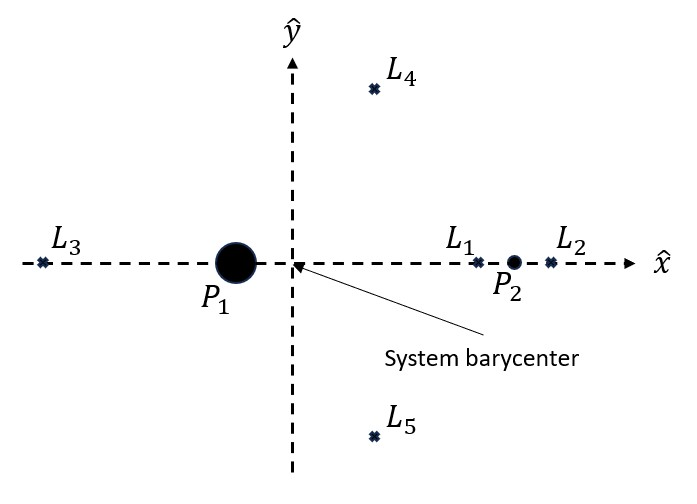
\includegraphics[width=0.5\textwidth]{figures/RotFrame.jpg}
    \caption{CR3BP barycentric rotating frame with Lagrange points.}
    \label{fig:rotFrame}
\end{figure}
